\section{\dpalt Heuristic for \spp}
\label{sec:swapping_efficient}

The DP-based algorithms presented in~\cite{tqe22-quantum} for the \spp problem
have high time complexity, and thus, may not be practical for real-time route finding in large networks. In this section, we develop an almost-linear time 
heuristic for the \spp problem, based on the classic Dijkstra shortest
path algorithm; the designed heuristic performs close to the DP-based algorithms
in our empirical studies.

\para{Basic Idea.}
The main reason for the high-complexity of our DP-based algorithms
in~\cite{tqe22-quantum} is that
the goal of the \spp problem is to select an optimal swapping \textit{tree} 
rather
than a path. One way to circumvent this challenge efficiently while still
selecting near-optimal swapping tree, is to restrict ourselves to only 
``balanced'' swapping trees. This restriction allows us to think in terms
of selection of paths---rather than trees---since each path has a unique\footnote{In fact, there can be multiple balanced trees over a path whose length is not a power of 2, but, since they differ minimally in our context,
we can pick a unique way of constructing a balanced tree over a path.}
balanced swapping tree.
%%%%%%%%%%%%%
We can then develop an appropriate path metric based on above, and design
a Dijkstra-like algorithm to select an $(s,d)$ path that has the optimal
metric value.
%%%%%%%%%%%%%%%%%
We note that Caleffi~\cite{caleffi} also proposed a path metric based on 
balanced swapping trees, but their metric, though accurate, only had a
recursive formulation without a closed-form
expression---and hence, was ultimately not useful in designing an efficient
algorithm. In contrast, we develop an approximate
metric with a closed-form expression, 
based on the "bottleneck" link, as follows.

\para{Path Metric $M$.}
Consider a path $P = (s, x_1, x_2, \ldots, x_n, d)$ from $s$ to $d$,
with links $(s,x1), (x1, x2), \ldots, (x_n, d)$ with given \eps latencies.
We define the path metric for path $P$, $M(P)$, as the 
\eps generation latency of a balanced swapping over $P$, 
which can be estimated as follows.
%%%%%%%%
Let $L$ be the link in $P$ with maximum generation latency. 
%%%%%%%%%
If $L$'s depth (distance from the root) is the maximum in a throttled 
swapping tree, then we can easily determine the accurate generation 
latency of the tree. However, in general, $L$ may not have 
the maximum depth, in which case we can still estimate the tree's latency 
approximately, if the tree is balanced, as follows.
%%%%%%%%%%
In balanced swapping trees, \textit{assuming} the maximum latency link $L$
to be at the maximum depth, gives us a constant-factor approximation 
of the tree's generation latency. Thus, let us assume $L$ to be at 
the maximum depth of a balanced tree over $P$; this maximum depth
is $d = \lceil(\log_2 |P|)\rceil$.
%%%%%%%%%%%%%%
Let the generation latency of $L$ be $T_L$.
%%%%%%%%%%%%%%%%%%%%
If we ignore the $\bt + \ct$ term in
Eqn.~\ref{eqn:swapping_tree-rate}
% Eqn.~\ref{eqn:tree-rate}, 
, then, the generation latency of a throttled swapping tree can be 
easily estimated to $T (\frac{3}{2\bp})^d.$ 
%%%%%%%%%%%%%%%%%%
The term $\bt + \ct$  can also be incorporated as follows. 
Let $T(i)$ denote the expected latency of the ancestor of $L$ 
at a distance $i$ from $L$. Then, we get the recursive equation:
$T(i) = (\frac{3}{2}T(i-1) + \bt + \ct) / \bp.$
%%%%%%%%%%%%%
Then, the path metric value $M(P)$ for path $P$ is given by 
$T(d)$, the generation latency of the tree's root at a distance
of $d$ from $L$, and is equal to: 
$$M(P) = T(d) =\pp^{d}T_L + [(\pp^{d}-1) / (\pp-1)](\bt + \ct)/\bp$$ where 
$\pp = 3/(2\bp)$ and $d = \lceil(\log_2 |P|)\rceil$.
The above is a (1+3/(2\bp))-factor approximation latency 
of a balanced and throttled swapping tree over $P$.
%this can be shown easily using analysis from \S\ref{sec:swapping_dec}.

\para{Optimal Balanced-Tree Selection.}
The above path-metric $M()$ is a monotonically increasing function over 
paths, i.e., if a path $P_1$ is a sub-sequence of another path $P_2$, 
then $M(P_1) \leq M(P_2)$. Thus, we can tailor the classical Dijkstra's shortest path
algorithm to select a $(s,d)$ path with minimum $M(P)$ value, 
using the link's \eps generation
latencies as their weights. We refer to this algorithm
as \dpalt, and it can be implemented with a time complexity of 
$O(m + n \log n)$ using Fibonacci heaps, where $m$ is the number of edges 
and $n$ is the number nodes in the network. 

\para{Incorporating Fidelity Constraints.}
\begin{definition}
    Given a swapping tree, the total time spent by a qubit in a swapping
    tree is the time spent from its ``birth'' via an atom-photon \eps generation at a node till its consumption
    in a swapping operation or in generation of the tree's root \eps. 
    We refer to this as a qubit's \textit{age}. The maximum age over all qubits 
    in a swapping tree is called the tree's (expected) \textit{age}. See Fig.~\ref{fig:swapping_age}.
\end{definition}

\begin{figure}
    \centering
    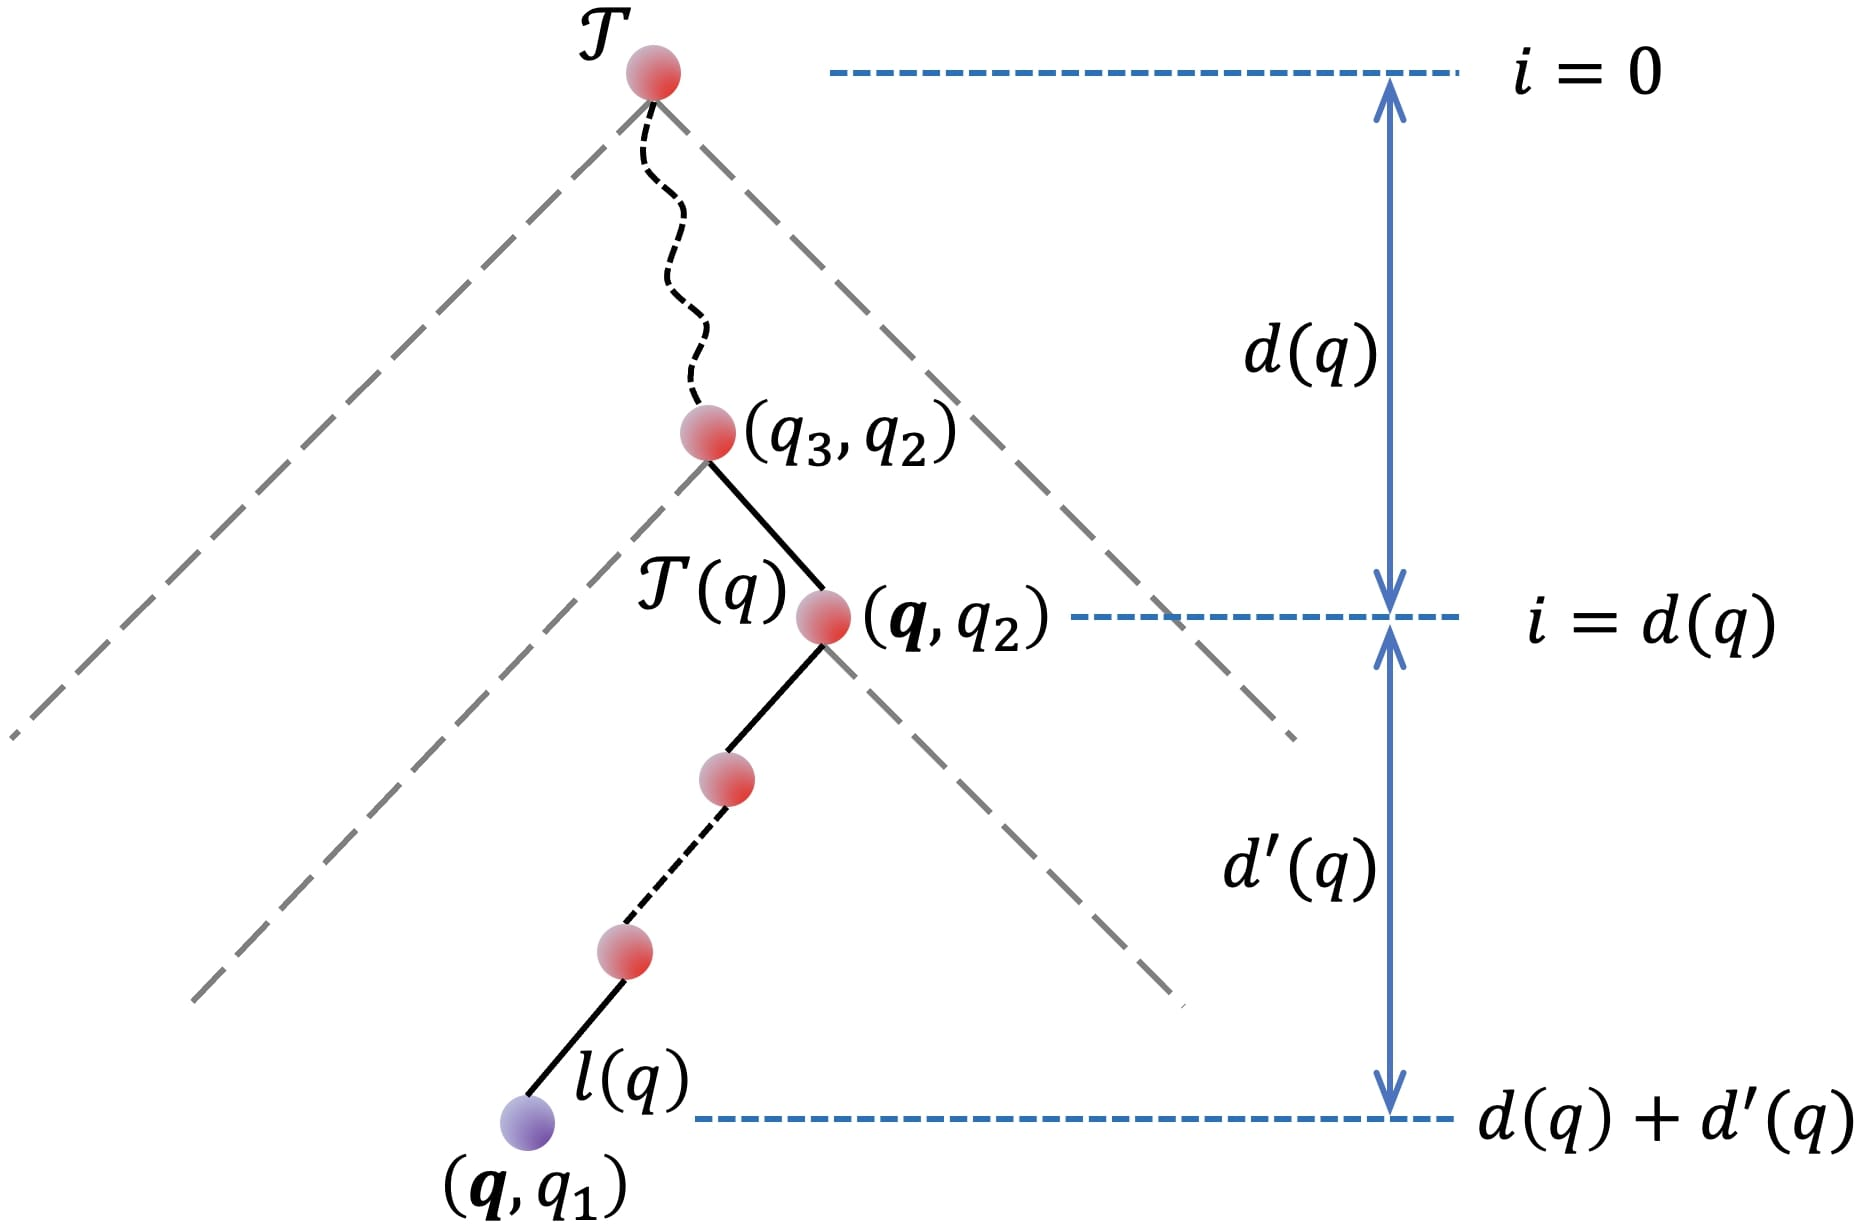
\includegraphics[width=0.7\textwidth]{chapters/swappingtrees/figures/qubit-age.jpg}
    % \vspace{0.1in}
  \caption{Qubit parameters in a swapping tree used to compute the \emph{age} of a qubit $q$ at a leaf node $l(q)$. Here, $l(q)$ is the left-most leaf of the subtree $\T(q)$.}
%   \vspace{-0.2in}
  \label{fig:swapping_age}
\end{figure}

Fidelity constraints in our path-metric based setting can be handled by essentially
computing the optimal path for each path-length (number of hops in the path) up to
$\fidl$, and then pick the best path among them that satisfies the fidelity constraints.
%%%%%%%%%%
This obviously limits the number of leaves to \fidl and addresses the operations-based
fidelity degradation. The above also address the decoherence/age
constraint, since it is easy to see %(from analysis in \S\ref{sec:swapping_dec}) 
that the age of a balanced swapping tree can be very closely 
approximated in terms of the latency and the number of leaves.
%%%%%%%%%%%%%%%
Now, to compute the optimal path for each path-length, we can use a simple dynamic
programming approach that run in $O(m\fidl)$ time where $m$ is the number of edges 
and $\fidl$ is the constraint on number of leaves. 